\documentclass[main]{subfiles}

\begin{document}

\begin{figure}
  \centering
  \begin{tikzpicture}[auto, node distance = 0.5cm and 0.5cm,every node/.style={inner sep=0pt}]
    \tikzset{A/.style={arrows={Circle-Stealth},draw,blue,ultra thick}}
    \node (login) {
\includegraphics[width=3cm]{images/android-login}};
    
    \node [below=of login] (main) {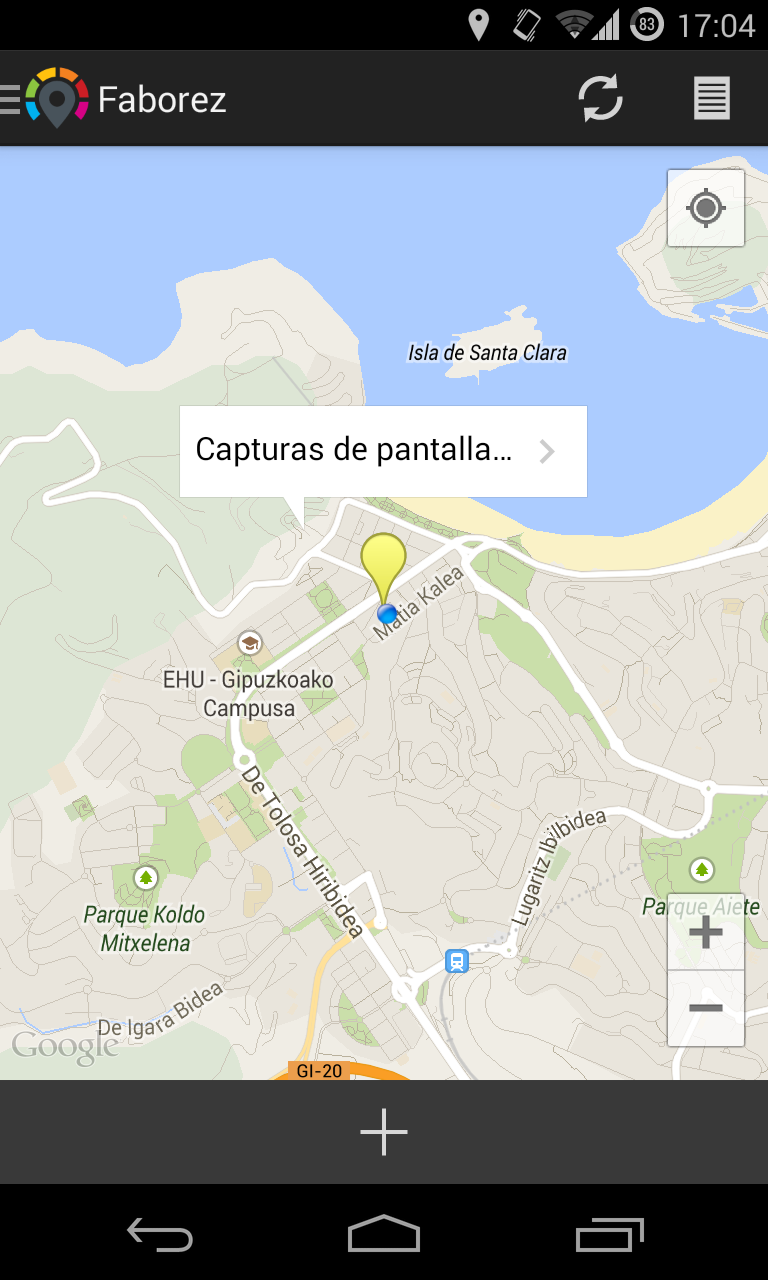
\includegraphics[width=3cm]{images/android-main-map}};
    \node [left=of main] (main-menu) {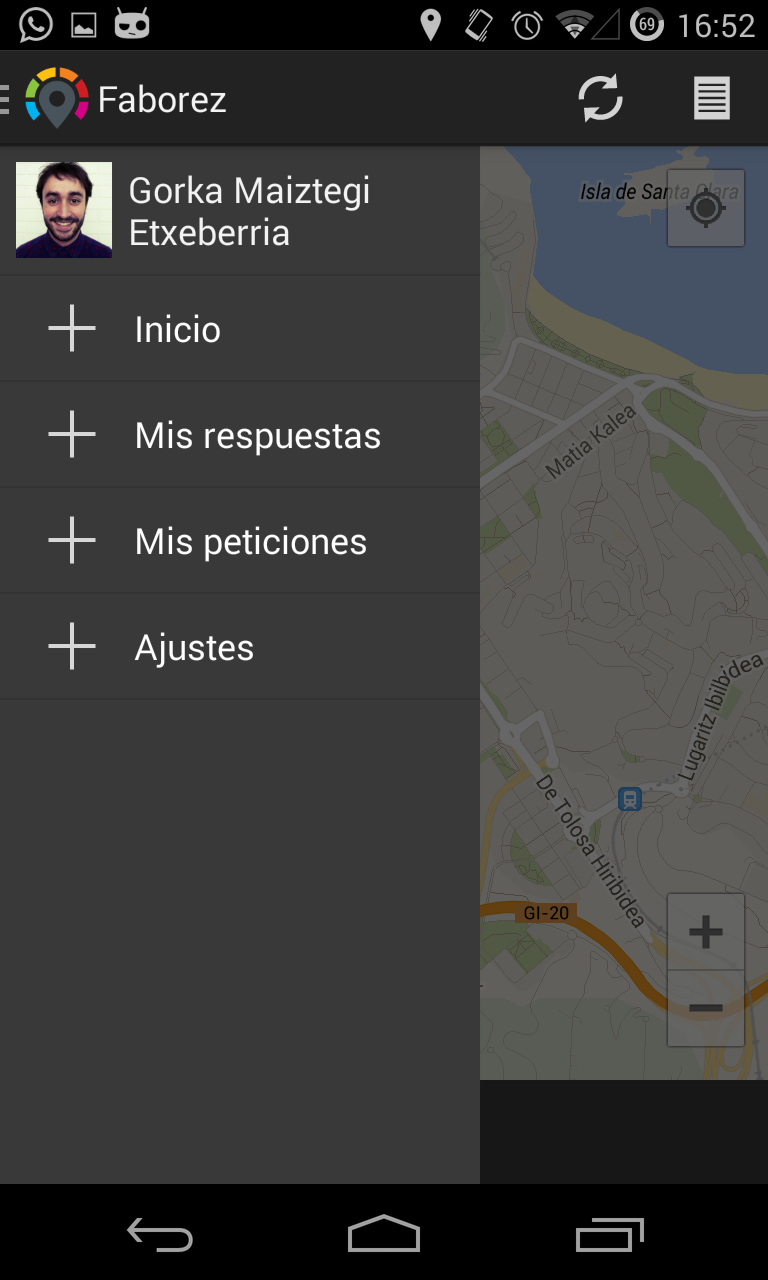
\includegraphics[width=3cm]{images/android-main-menu}};
    \node [right=of main] (main-right) {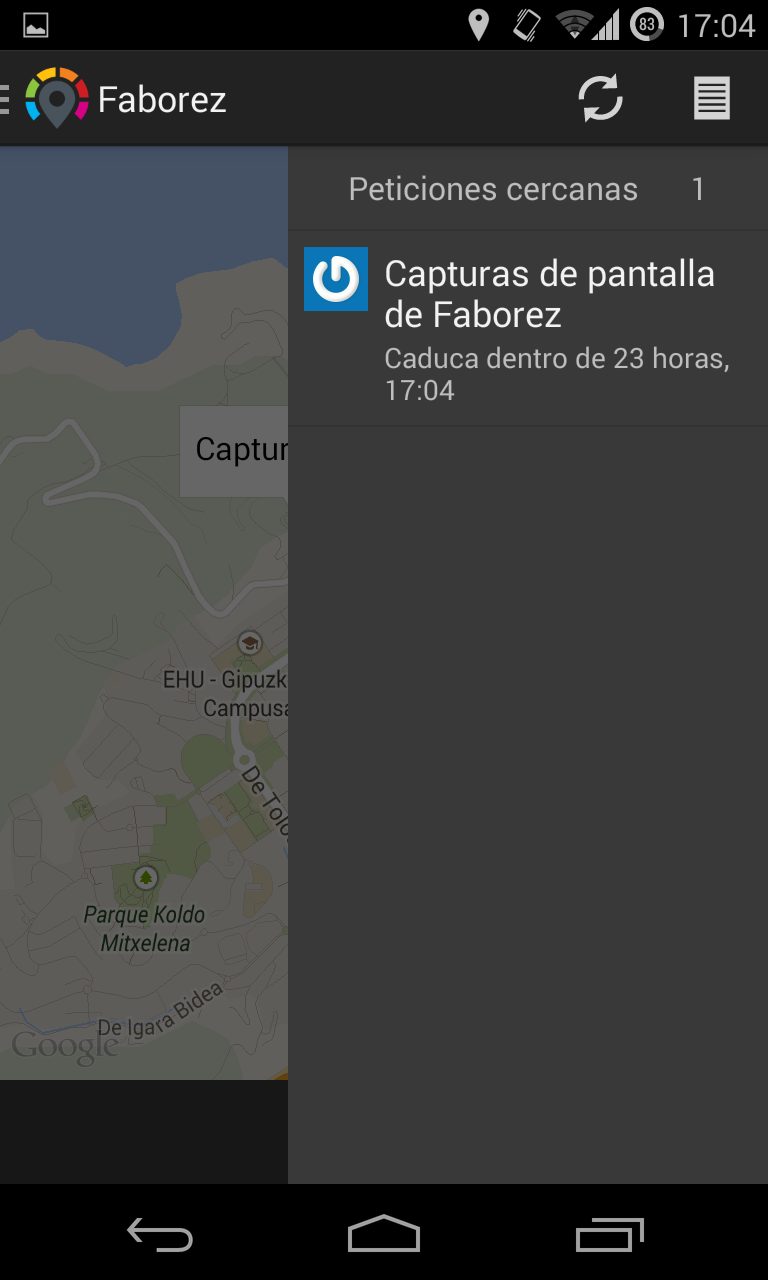
\includegraphics[width=3cm]{images/android-main-right}};
    \node [left=of main-menu] (settings) {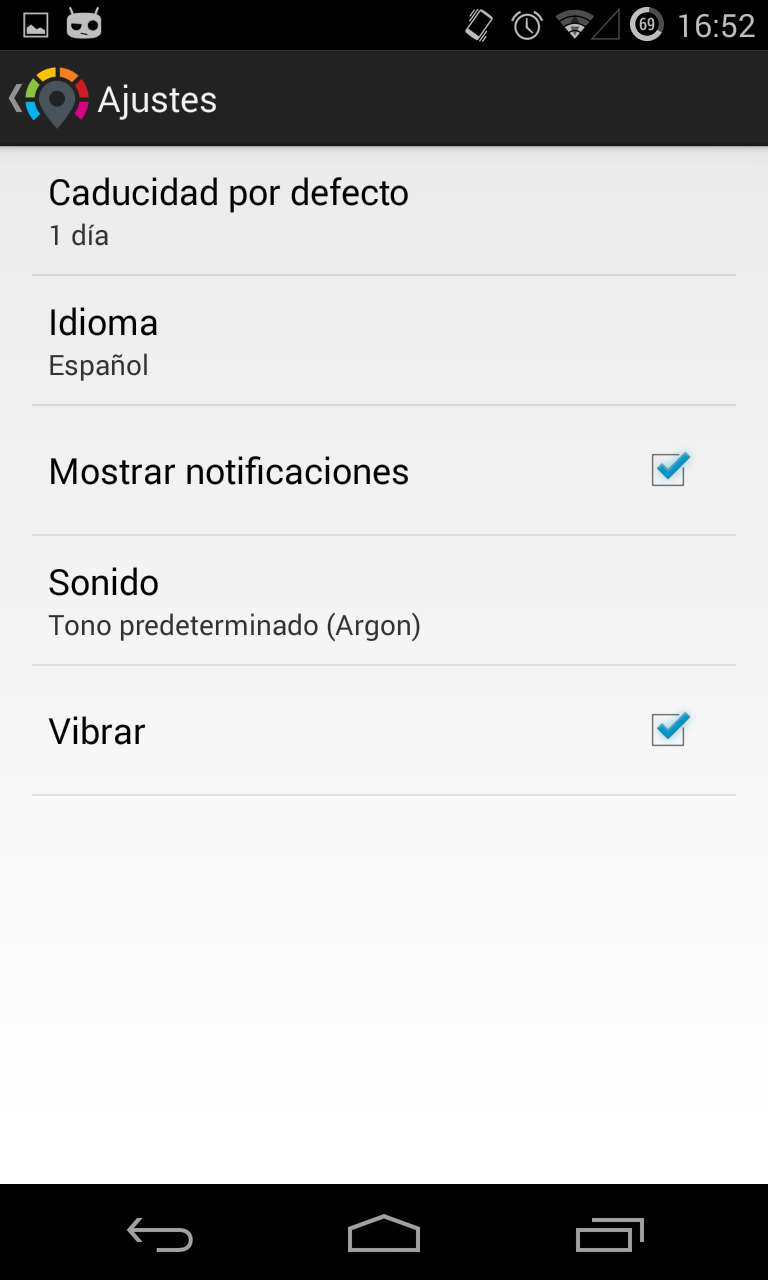
\includegraphics[width=3cm]{images/android-settings}};
    
    \node [below=of main-menu] (my-requests) {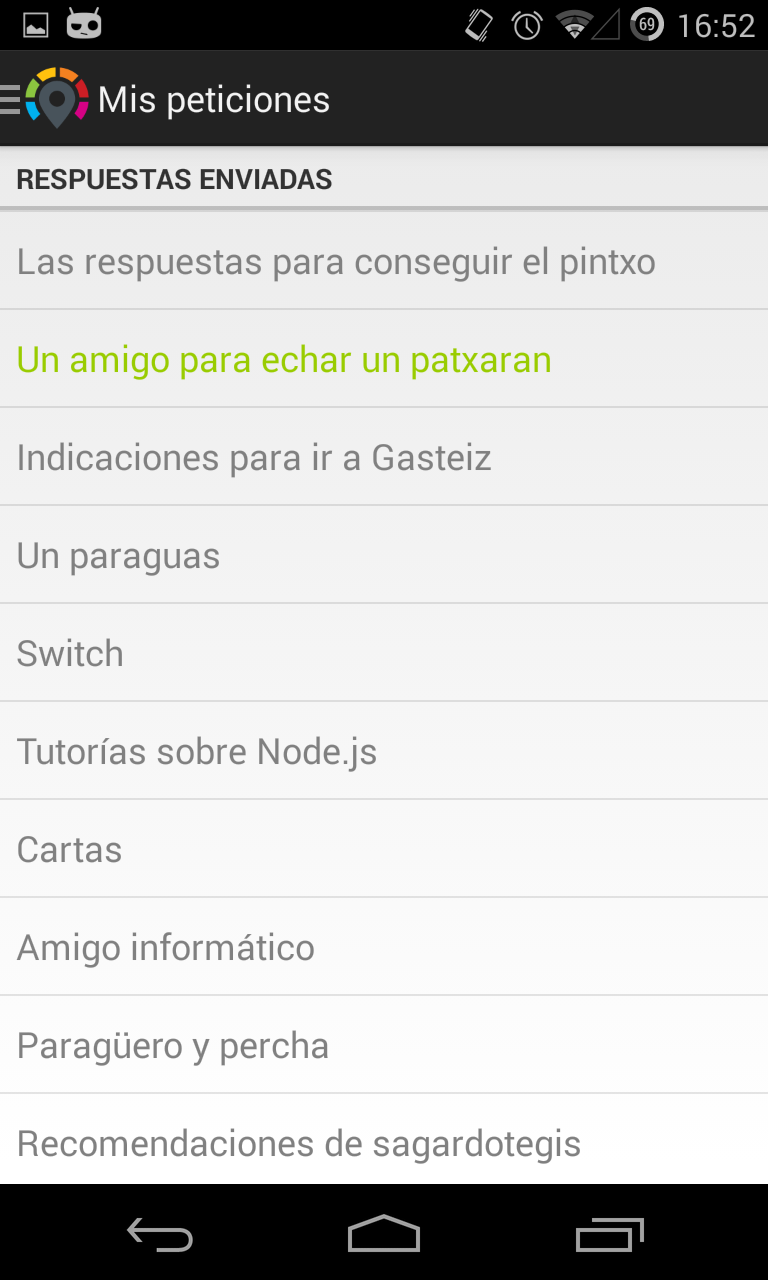
\includegraphics[width=3cm]{images/android-myrequests}};
    \node [below=of my-requests] (my-replies) {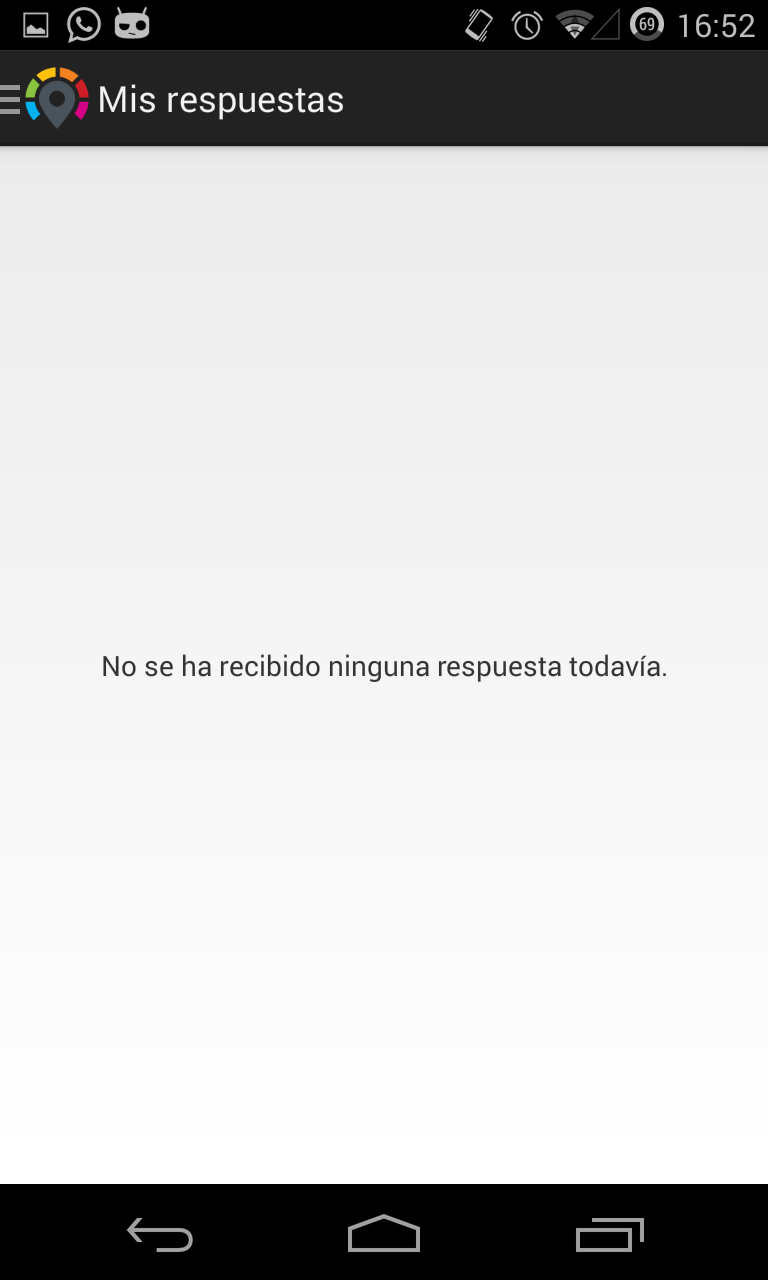
\includegraphics[width=3cm]{images/android-myreplies}};
    
    \node [below=of main-right] (request) {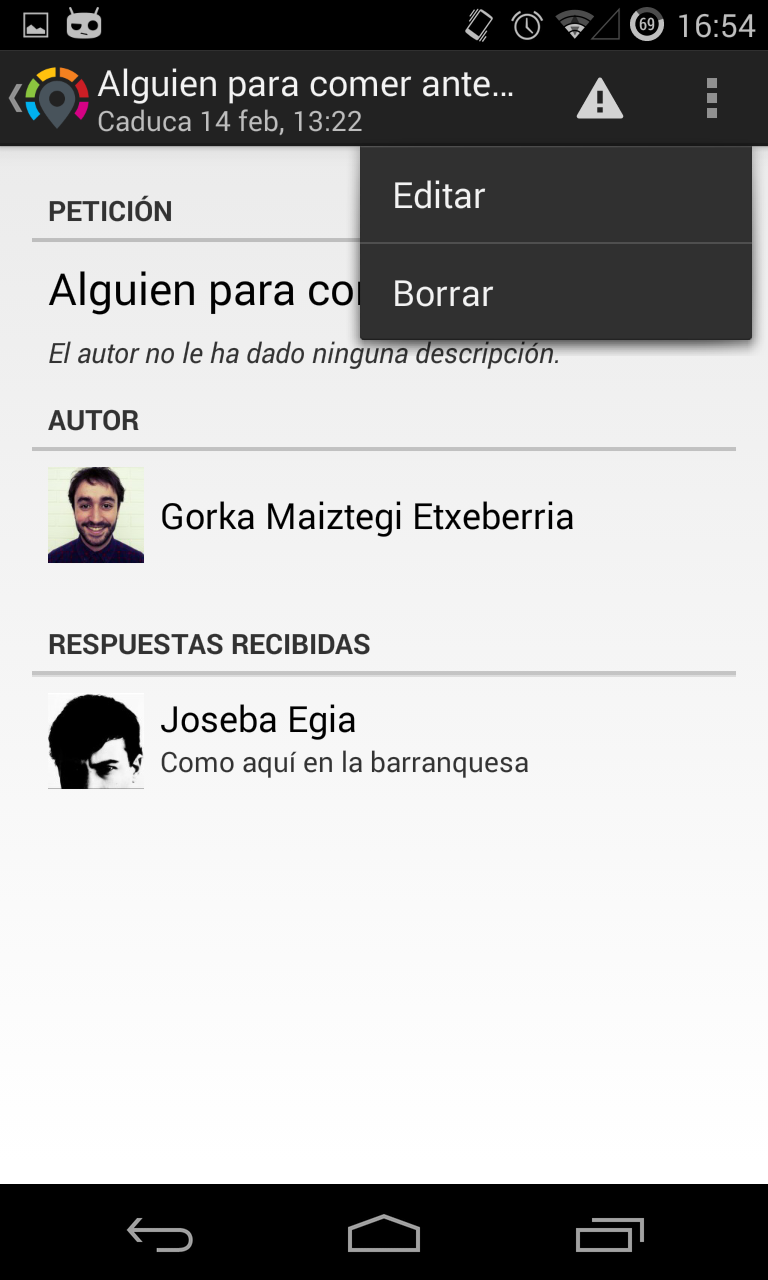
\includegraphics[width=3cm]{images/android-request}};
    
    \node [below=of main] (new-request) {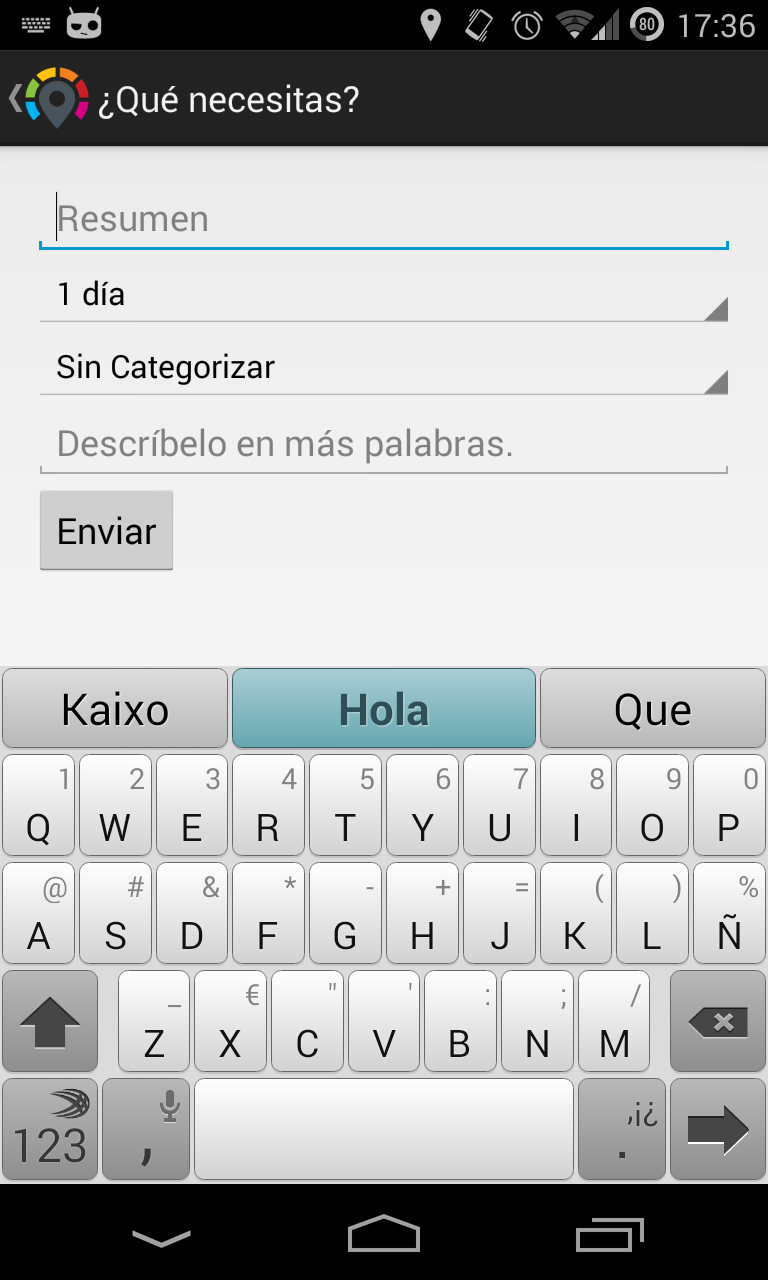
\includegraphics[width=3cm]{images/android-newrequest}};
    \node [below=of request] (reply) {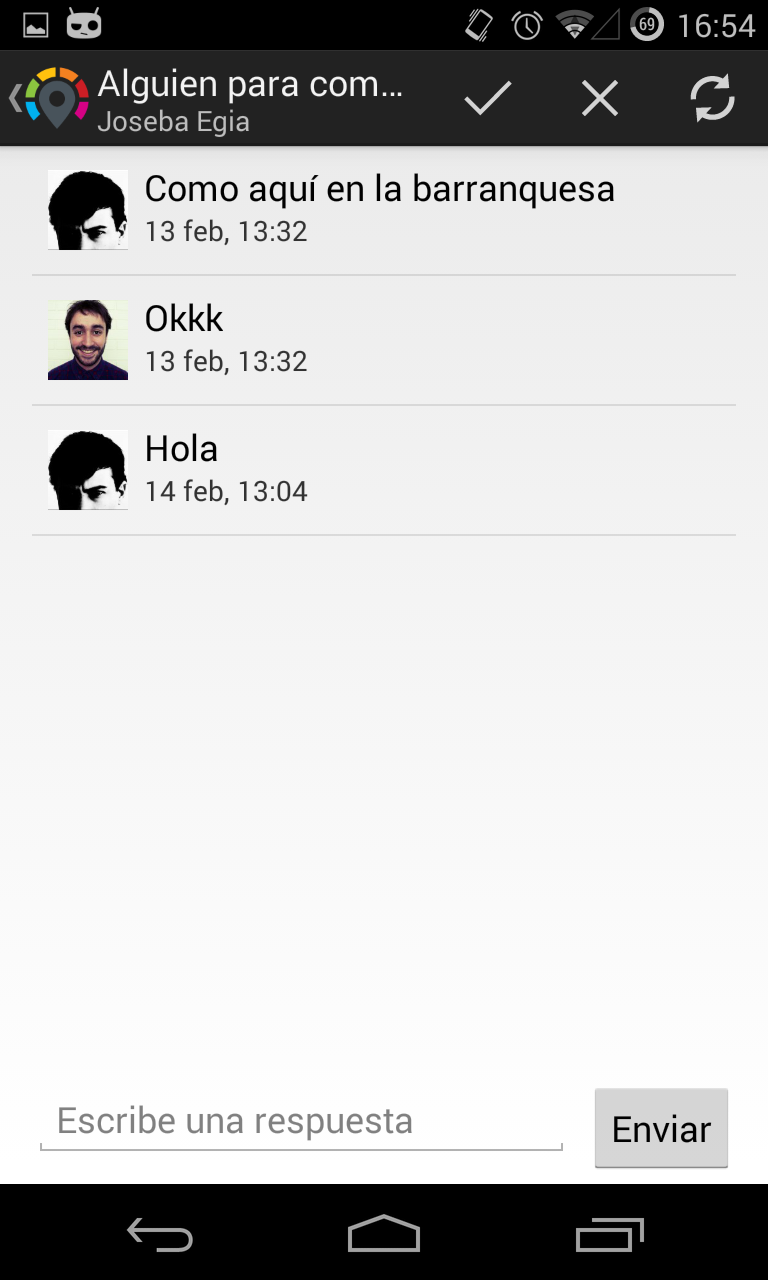
\includegraphics[width=3cm]{images/android-reply}};
    
    \draw [A] ($(login.north) !0.5! (login.south)$) -- (main);
    
    \coordinate (menu-open) at ($(main.north west) + (0.25,-0.45)$);
    \coordinate (right-open) at ($(main.north east) - (0.25,0.45)$);
    \coordinate (main-plus) at ($(main.south) + (0,0.7)$);
    \coordinate (map-infowindow) at ($(main) + (0,0.8)$);
    \draw [A] (menu-open) -- (main-menu.east |- menu-open);
    \draw [A] (right-open) -- (main-right.west |- right-open);
    \draw [A] (main-plus) -- (new-request);
    \draw [A] (map-infowindow) -- (request.north west);
    
    \coordinate (right-request) at ($(main-right) + (0.5,1.2)$);
    \draw [A] (right-request) -- (right-request |- request.north);
    
    \coordinate (menu-replies) at ($(main-menu) - (0.5,-1)$);
    \coordinate (menu-requests) at ($(main-menu) - (0,-0.5)$);
    \coordinate (menu-settings) at ($(main-menu) - (1,0)$);
    \draw [A] (menu-replies) -- (my-replies.north -| menu-replies);
    \draw [A] (menu-requests) -- (my-requests.north -| menu-requests);
    \draw [A] (menu-settings) -- (settings.east |- menu-settings);
    
    \coordinate (request-item) at ($(my-requests)$);
    \draw [A] (request-item) -- (request.west |- request-item);
    
    \draw [A] (my-replies.center) -- (reply);
    
    \coordinate (newrequest-send) at ($(new-request) - (1.3,-0.3)$);
    \draw [A] (newrequest-send) -- (newrequest-send -| request.west);
    
    \coordinate (request-reply) at ($(request) - (0,0.3)$);
    \draw [A] (request-reply) -- (reply);
    
  \end{tikzpicture}
  \caption{Las pantallas de la interfaz de usuario y el movimiento entre ellas}
  \label{fig:activity-relations}
\end{figure}

\end{document}
